\documentclass[cover.tex]{subfiles}


\begin{document} \begin{refsection}


%%%%%%%%%%%%HEADING TITLE
\hfill
\vspace{0.2cm}
\begin{center}
{\large \bfseries 
EXPERIMENT 
\par
\Huge
Molecular Geometry
\\[5pt] \par}
\vspace{0.2cm}
\end{center}
\par
\noindent
%\uline{  \hfill \normalsize \hfill       }
%%%%%%%%%%%%HEADING
\section*{Goal}
This experiment will go over the ideas of molecular geometry and bond-hybridization. On one hand, you will learn how to predict the geometry of a molecule and how to differentiate, for example, a linear molecule from a bent molecule. Also you will learn to predict the hybridization of atomic orbitals involved in a chemical bond.
\section*{Materials}
This is a theory-based experiment. You will not carry any lab work during this experiment and you only need a molecular models kit. 
\section*{Background}
Molecules result from the combination of atoms. For example, a \ce{H2O} molecule results of the combination of one oxygen atom with two hydrogen atoms. The atoms of a molecule combine by exchanging or sharing electrons, depending on the type of bond. Water is a covalent molecule and the oxygen and hydrogen atoms share the electrons in the bond. Only electrons in the outermost electron shell participate in chemical bonds. Those electrons are called \text{valence electrons}. Core electrons, electrons in inner shells of the atom, do not participate in chemical bonds. The electron configuration of oxygen is $1s^2$\textbf{$2s^2 2p^4$}. Valence electrons are highlighted with bold letters and are those in the energy level $n=2$. Chemists use several theories to describe the formation of a bond, and here we will cover three of these theories: the valence-shell electron-pair repulsion model (VSEPR), the valence bond theory, and the molecular orbital theory. These theories describe different aspects of the formation of a bond, sometimes complementing each other.


\subsection*{Valence Electrons}
The valence electrons of an atom are those located in the electronic valence shell. For example, the electron configuration of lithium is $1s^2 2s^1$. This atom has two electrons in the $1s$ atomic orbital and one electron in the $2s$ higher-energy atomic orbital. The first two electrons belongs to the core, as the level $1s$ is completely filled with electrons. Differently, the second energy level is not completely filled and hence the single electron in this level is a valence electron. Another example would be oxygen,$1s^2 2s^2 2p^4$, which contains two core electrons--located in the $1s$ level--and six valence electrons. The number of valence electrons of an atom can be easily determine by looking at the group number. For example, oxygen belongs to the group 16(6A) and has six valence electrons. Similarly, nitrogen belongs to group 15(5A) and hence will have five valence electrons.
\subsection*{The Octet rule} Atoms gain or loose electrons when they combine to form molecules. The octet rule says that each atom in a molecule is surrounded by eight electrons. There are two important exceptions to this rule: hydrogen (\ce{H}) will only surrounded by two electrons, and boron (\ce{B}) by six.
\subsection*{Lewis dot symbol of an atom}
The Lewis dot symbol of an atom is a representation of the element symbol surrounded by the valence electrons in the form of dots. For example, Li has one valence electron and hence its Lewis dot symbol will be \hspace{0.1cm}\lewis{4.,Li}\hspace{0.1cm}. The Lewis dot symbol for O, with six valence electrons, will be \hspace{0.1cm}\lewis{0.2:4.6:,O}\hspace{0.1cm}. At this point is not that important how do you distribute the dots, and in case of doubt a wise choice is to pair the dots.

\subsection*{Lewis structure of diatomic molecules}
In order to build up Lewis structures or electron-dot structures for diatomic molecules, 
\begin{enumerate} 
\item set up the element symbols next to each other. 
\item count the total number of valence electrons in the molecule, by adding the valence electrons of each atom. 
\item Add as many electrons (dots) as necessary to complete the octets (or duets) for each element. Make sure that there are at least two electrons shared (a single bond) between the two elements. 
\item Count how many electrons are used in the resulting structure
\begin{enumerate}
\item If the structure uses as many electrons as valence electrons are available, this is the final structure.
\item If the structure uses more electrons than valence electrons are available, double bonds (four electrons shared) or triple bonds (six electrons shared) need to be used. Each double bound will save two electrons with respect to a single bond. Each triple bound will save two electrons with respect to a double bound.
 \end{enumerate}
 \end{enumerate}
 
\subsection*{Lewis structures of polyatomic molecules}
For polyatomic molecules the procedure is exactly the same. The only difference is to arrange the elements correctly. Typically, finding the central atom is the key. Two tricks to find the central atom.
\begin{enumerate}
\item the central atom is the one with a lower index in the molecule (e.g. in \ce{H2O} is \ce{O} or in \ce{NH3} is \ce{N})
\item the central atom is that with the lowest electronegativity.
\end{enumerate}
The pairs of electrons that connect two atoms are called \begin{it}bonds\end{it}. In Lewis structures these two electrons can be replaced by lines joining the elements. The pairs not involved in a bond are called \begin{it}lone pairs\end{it}. Notice that the atoms arrangement (if the structure looks like a line, a triangle or so) is not necessary representative of the real, three-dimensional molecular geometry.
 
 %%%%%%%%%EXAMPLE BOX%%%%%%%%%%
\begin{example}{Example}
\begin{it} 
Construct the electron-dot structure of \ce{H2O} indicating the number of bonds and lone pairs.
\end{it}\\
\Sepline
\begin{bf}Answer\end{bf}: we first arrange the atoms in the molecule as \ce{H}\hspace{.05in}\ce{O}\hspace{.05in}\ce{H}. The central atom is \ce{O}, as oxygen has the lower index in the \ce{H2O} molecule--the index for O is one and the index for H is two. Now we count the total number of valence electrons, including all atoms: 2xH(1$e^-$) and O(6$e^-$) that gives a total of eight electrons. Now we distribute the pair on each atoms knowing that each atom has to have 8 electrons with the exception of hydrogen that can only be surrounded by two.
\begin{center}\lewis{0:,H}\hspace{.05in}\lewis{2:6:,O}\hspace{.05in}\lewis{4:,H}\hspace{.05in}\end{center} 
and using lines instead of pairs (this is not necessary but makes the electron-dot structure look better) we obtain
\begin{center}\chemfig{ H-[:0]\lewis{2:6:,O}-H}\hspace{.05in} \end{center}
The molecule has two bonds, each one connecting a H to the oxygen atom, and two lone pairs located on the oxygen atom.
\end{example}
%%%%%%%%%EXAMPLE BOX%%%%%%%%%%

\subsection*{Atomic charges in a molecule and polyatomic ions}
In order to build up the electron-dot structures of a molecule you need to count the number of valence electrons of the whole molecule. Each atom contributes with a different number of valence electrons to the molecule. For example, H contributes with one electron whereas O contributes with two. When you arrange the electron pairs in the molecule, each atom should have no less than the number of electrons that they bring. For example in the electron-dot structure of HCl, \lewis{0:,H}\hspace{.05in}\lewis{0:2:6:,Cl}\hspace{.05in} the hydrogen atom contributes with one electron to the molecule, and in the molecule the H atom owns one electron, as in \lewis{0:,H}\hspace{.05in}  one of the dots belongs to \ce{H} and the other belongs to the \ce{Cl}--the electrons are shared in a covalent bond. In the same way, the \ce{Cl} atom contributes with seven electrons and in the molecule it owns seven electrons, as in \lewis{0:2:4:6:,Cl}\hspace{.05in} one of the dots belongs to \ce{H} and the other seven belong to \ce{Cl}. In another words, the \lewis{0:,H}\hspace{.05in}\lewis{0:2:6:,Cl}\hspace{.05in} electron-dot structure is the combination of \lewis{0.,H}\hspace{.05in} and \hspace{.05in}\lewis{0:2:4.6:,Cl}\hspace{.05in}. We say that the charges on each atom are zero, as each atom in the molecule owns the same number of electrons that it originally brings. The lewis structure should also display the electron distribution in polyatomic ions. Look for example at \ce{CH3^-} ions. Comparing the valence electrons of each atom and the number of electrons surrounding each atom in this structure, one can see that the C atom has an extra electron, and hence it is responsible of the negative charge:
\begin{center}
\chemfig{\chemfig{\circleatom{\lewis{2:,C^{-}}}( (-[:0]H)(-[:180]H)(-[:270]H))}}  % I want 
\end{center}



\subsection*{VSEPR theory and molecular geometry}
Molecules are arrangements of atoms, and these arrangements can have different forms. Think about a \ce{H2O} molecule, which contains two hydrogen atoms and one oxygen. Knowing that both hydrogens are connected to oxygen by means of a covalent bond, one can envision several molecular geometries such as 
\begin{center}
\chemfig{ H-[:0]\lewis{2:6:,O}-H}\hspace{.05in} or \hspace{1cm} maybe \hspace{1cm} \chemfig{H-[:52.24]\lewis{1:3:,O}-[::-104.48]H}
\end{center} 
The goal of this section is to identify the geometry of a given molecule. In order to do this, the electron-dot structure of the molecule is the key. If the molecule contains two atoms, there is only a possible geometry these two atoms can exhibit, and this is a linear arrangement. For the case of more complex molecules, in order to identify the geometry you need to figure out the ABE code of the molecule. In this code B refers to the number of atoms connected to the central atom in a molecule, and E is the number of lone pairs on the central atom. For example, the electron-dot \hspace{.05in}\chemfig{ H-[:0]\lewis{2:6:,O}-H}\hspace{.05in} structure has two bonds with the central atom \ce{B2} and two lone pairs on top of the central atom \ce{E2} and hence the ABE code of the molecule would be \ce{AB2E2}. Another example, the ABE code for  ammonia  \begin{center} \chemfig{\lewis{2:,N}( (-[:0]H)(-[:180]H)(-[:270]H))} \end{center}  
would be \ce{AB3E}, as the molecule has three atoms connected to the central nitrogen and and \ce{N} has a single lone pair. You can find a list of the equivalence between ABE codes and the molecular geometry in Table 1. In order to predict the geometry of a molecule, once you have the ABE code, Table 1 will give you the geometry. For example, an \ce{AB2} molecule will be linear, whereas an \ce{AB2E2} is a bent. The bond angles are also indicated in the table, and for example a \ce{CO2} molecule, which will be linear, will have 180$^{\circ}$ angles. This means both C-O bonds will form a line.

%\clearpage
\begin{center}
\begin{minipage}{0.5\textwidth}

\captionof{table}{Molecular Geometries}%\fontfamily{ppl}\selectfont
\begin {table}[H]
 \label{tab:vsepr}
 \begin{tabular}{llll}
%\rowcolor{black!45}
\toprule
ABE Code & Molecular shape & Bond Angle & 3D model   \\
\midrule
\ce{AB2} &  Linear      &  $180^{\circ}$    &   \begin{minipage}{.1\textwidth}\includegraphics[width=15mm, height=15mm]{./geometry/geom1}\end{minipage}   \\

\ce{AB3E} &  Trigonal pyramidal    &  $109^{\circ}$    &   \begin{minipage}{.1\textwidth}\includegraphics[width=15mm, height=15mm]{./geometry/geom5}\end{minipage} \\
\ce{AB3} &  Trigonal Planar      &  $120^{\circ}$    &   \begin{minipage}{.1\textwidth}\includegraphics[width=15mm, height=15mm]{./geometry/geom2}\end{minipage}\\

\ce{AB2E2} &  Bent    &  $109^{\circ}$    &   \begin{minipage}{.1\textwidth}\includegraphics[width=15mm, height=15mm]{./geometry/geom6}\end{minipage}\\
\ce{AB2E} &  Bent      &  $120^{\circ}$    &   \begin{minipage}{.1\textwidth}\includegraphics[width=15mm, height=15mm]{./geometry/geom3}\end{minipage}\\

\ce{AB5} &  Trigonal bipyramidal    &  $90^{\circ}$, $120^{\circ}$,$180^{\circ}$    &   \begin{minipage}{.1\textwidth}\includegraphics[width=15mm, height=15mm]{./geometry/geom7}\end{minipage}\\
\ce{AB4} &  Tetrahedral      &  $109^{\circ}$    &   \begin{minipage}{.1\textwidth}\includegraphics[width=15mm, height=15mm]{./geometry/geom4}\end{minipage} \\

 \ce{AB6} &  Octahedral   &  $90^{\circ}$, $180^{\circ}$,$180^{\circ}$    &   \begin{minipage}{.1\textwidth}\includegraphics[width=15mm, height=15mm]{./geometry/geom8}\end{minipage}\\
\bottomrule
 
\end{tabular}
\end{table}
\end{minipage}
\end{center}

\subsection*{Atomic orbitals}
There are four main types of atomic orbitals: s, p, d and f. Each orbital type has a specific symmetry. For example, s orbitals are spherical, whereas the p orbitals consist of two lobes on opposite sides of the nucleus.

\subsection*{Valence bond theory and hybrid orbitals}
The \emph{valence bond theory} is a qualitative model that describes the formation of the chemical bonds. It assumes that the electrons of a molecule are located in atomic orbitals, as if the atoms in the molecule where separate from each other. These valence orbitals combine to produce mixed orbitals, known as \emph{hybrid orbitals}. The mixing of orbitals is called \emph{orbital hybridization}. Examples for orbital hybridization are sp, sp$^2$, sp$^3$ or sp$^3$d. In the previous examples, s and p orbitals are mixed giving sp, sp$^2$ or sp$^3$ hybrid orbital. In the last case, sp$^3$, three p orbitals mix with a single s orbital, allowing for a total of four bonds. In the case of the sp$^3$d hybrid orbital, three p orbitals mix with a s and a d orbital allowing a total of five bonds.\\
Let us analyze the formation of hybrid orbitals for the case of methane, \ce{CH4}. Carbon has four valence electrons located in 2s and 2p orbitals,
% \begin{center}   \Large{C}\hspace{1cm}\electron{2s}{\updwn}\quad \electron{2p}{\up\ \up\ \emp} \hspace{1cm}\Large{H}\hspace{1cm}\electron{1s}{\up}\end{center}
each hydrogen has one valence electron located in a 1s orbital. When the C and H combine, the carbon atom transforms into a $sp^3$ hybrid, leading to four bonds. You can obtain the orbital hybridization in each atom by means of the ABE code. For example, an $AB_2E_3$ molecule will have five electron regions--resulting of adding the B's and the E's. Table 2 provides the equivalency between the ABE code and the orbital hybridization.\\


%%%%% ATOMIC ORBITALS
 \begin{figure}[ht!]
  \centering
  \begin{tikzpicture}
  \begin{scope}[font=\itshape]% to not type it every time, but better go for math mode
  \draw[-latex] (0,0)--(1,0) node[above]{x};
  \draw[-latex] (0,0)--(-0.5,-0.7) node[above]{y};
  \draw[-latex] (0,0)--(0,1) node[above]{z};
  \orbital[pos = {(0,0)}]{py}
  \node[above] at (0.7,0.7) {p$_x$};

  \draw[-latex] (3,0)--(4,0) node[above]{x};
  \draw[-latex] (3,0)--(2.5,-0.7) node[above]{y};
  \draw[-latex] (3,0)--(3,1) node[above]{z};
  \orbital[pos = {(3,0)}]{px}
  \node[above] at (3.7,0.7) {p$_y$};

  \draw[-latex] (6,0)--(7,0) node[above]{x};
  \draw[-latex] (6,0)--(5.5,-0.7) node[above]{y};
  \draw[-latex] (6,0)--(6,1) node[above]{z};
  \orbital[pos = {(6,0)}]{pz}
  \node[above] at (6.7,0.7) {p$_z$};
  
   \draw[-latex] (9,0)--(10,0) node[above]{x};
  \draw[-latex] (9,0)--(8.5,-0.7) node[above]{y};
  \draw[-latex] (9,0)--(9,1) node[above]{z};
\orbital[pos = {(9,0)}]{s}
  \node[above] at (9.7,0.7) {1s};
  
     \draw[-latex] (12,0)--(13,0) node[above]{x};
  \draw[-latex] (12,0)--(11.5,-0.7) node[above]{y};
  \draw[-latex] (12,0)--(12,1) node[above]{z};
\orbital[scale = 1.5, pos = {(12,0)}]{s}
  \node[above] at (12.7,0.7) {2s};
  
  \end{scope}
  \node[minimum width=\columnwidth] at (current bounding box.center){};  
    \end{tikzpicture}
    \begin{tikzpicture}
\atom[name=C, color=blue, scale=1.2]{blue/90/north/1,
blue/0/east/1,
blue/270/south/1,
blue/180/west/1}
\atom[name=H, color=gray, pos={(0,1.8)}, scale=.8]{gray/270/south/1}
\atom[name=H, color=gray, pos={(1.8,0)}, scale=.8]{gray/180/west/1}
\atom[name=H, color=gray, pos={(-1.8,0)}, scale=.8]{gray/0/east/1}
\atom[name=H, color=gray, pos={(0,-1.8)}, scale=.8]{gray/90/north/1}
\end{tikzpicture}
\begin{tikzpicture}
\atom[name=B, color=blue, scale=1.2]{blue/0/east/1,
blue/120/north/1,
blue/240/south/1}
\atom[name=H, color=gray, pos={(-0.9,1.5)}, scale=.9]{gray/-45/-45/1}
\atom[name=H, color=gray, pos={(1.9,0)}, scale=.9]{gray/180/180/1}
\atom[name=H, color=gray, pos={(-0.8,-1.6)}, scale=.9]{gray/55/55/1}
\end{tikzpicture}
  \caption{Atomic orbitals of an oxygen atom. From left to right: p$_x$, p$_y$, p$_z$, 1s and 2s. (Bottom left) Hybrid sp$^3$ orbitals in \ce{CH4} resulting of the combination of three p orbitals and the s orbital of C and bonding the s orbitals of hydrogen. (Bottom right) Hybrid sp$^3$ orbitals in \ce{BH3}.}   
 \end{figure}

Another example would be \ce{BH3}. The chemical bond in this molecule results from the hybridization of boron s orbital with the two p orbital giving a sp$^2$ hybridization. As the class of the molecule is AB$_3$, it has three electron regions. Indeed, according to Table 2, an AB$_3$ has sp$^2$ hybridization.

\begin{minipage}{0.5\textwidth}
\begin{center}
\fontfamily{ppl}\selectfont
\captionof{table}{Equivalency between the ABE code and the orbital hybridization.}%\fontfamily{ppl}\selectfont
\begin{tabular}{lccp{3cm}lc}
%\rowcolor{black!45}
\toprule
ABE Code & Electron Regions & Hybrid & Shape&Bond Angle  \\
\midrule
\ce{AB2}, \ce{ABE} &  2     &  sp &\begin{minipage}{.1\textwidth}\begin{tikzpicture}
\satom[name=A, color=green!50!black]{red/180/180/0/1 ,red/0/0/0/1}
\end{tikzpicture}\end{minipage}   &   $180^{\circ}$  \\
\ce{AB3}, \ce{AB2E},\ce{ABE3} &  3    &  sp$^2$ &\begin{minipage}{.1\textwidth}  \begin{tikzpicture}
\satom[name=A, color=green!50!black]{red/180/180/0/1 ,red/25/25/0/0.8,red/-30/-30/0/0.9 }
\end{tikzpicture}
\end{minipage}   &   $120^{\circ}$  \\
\ce{AB4}, \ce{AB3E},\ce{AB2E2},\ce{ABE3}  &  4    &  sp$^2$ &\begin{minipage}{.1\textwidth}  
\begin{tikzpicture}
\satom[name=A, color=green!50!black]{red/90/90/0/1 ,red/-19/-19/0/.9, red/255/255/0/1, red/199/199/0/0.9}
\end{tikzpicture}
\end{minipage}   &   $109.5^{\circ}$  \\
\ce{AB5}, \ce{AB4E},\ce{AB3E2},\ce{AB2E3}  &  5    &  sp$^3$d &\begin{minipage}{.1\textwidth}  
\begin{tikzpicture}
\satom[name=A, color=green!50!black]{red/90/90/0/1,red/180/180/0/1 ,red/25/25/0/0.8,red/-30/-30/0/0.9,red/270/270/0/1 }
\end{tikzpicture}
\end{minipage}   &   $90^{\circ}$ and $120^{\circ}$  \\
\bottomrule
\end{tabular}
\label{tab:hybrid}\end{center}
\end{minipage}


\subsection*{Polarity of a molecule}
There are polar or non-polar bonds, and the concept of bond polarity is connected to the idea of \emph{electronegativity}. Some atoms in a covalent bond tend to attract more the bond-electrons than the others, and we call this atoms electronegative atoms. An example would be the case of a \ce{HF} molecule. H is an electropositive atom whereas F is electronegative. This means that in the bond, F will attract more the bond-electrons than H. This different tendency to attract the bond electrons created a dipole moment in the bond.\\
\begin{center}
\chemfig{
        \chemabove[3pt]{H}{\scriptstyle\delta +}(-[::270,0.5,,,draw=none]@{a})-
        \chemabove[3pt]{F}{\scriptstyle\delta -}(-[::270,0.5,,,draw=none]@{b})
        }
\chemmove{
          \draw[|->, very thick] (a)--(b);
         }
%         \qquad
%\chemfig{
%         \chemabove[3pt]{O}{\scriptstyle\delta -}(-[::270,0.5,,,draw=none]@{c})-
%         \chemabove[3pt]{H}{\scriptstyle\delta +}(-[::270,0.5,,,draw=none]@{d})
%        }
%\chemmove{
%          \draw[|->, very thick] (d)--(c);
%          }
\end{center}

The electronegativity is a periodic trend that increases from left to right and from bottom to top of the periodic table. Sometimes, these dipole moments in molecules due to the geometry cancel out and the molecule is non-polar as a whole. An example would be \ce{CO2}. Every C-O bond is polar, as oxygen is more electronegative than carbon. However, as the molecule is linear the C-O dipole moments cancel out each other and, over all, the molecule is non-polar.



%%%%%BIBLIOGRAPHY
%\printbibliography[heading=references,segment=\therefsegment]
%\printbibliography[segment=\therefsegment,heading=subbibliography]
\printbibliography[heading=subbibliography]
%%%%%BIBLIOGRAPHY



%\section*{Lab Information}
% \begin{itemize}[label={$\blacksquare$}]
%   \item  Duration \showclock{2}{30} : 2.30h
%   \item Related Topics: limiting reactant, excess reagent
%     \item Lab skills: gravimetry
% \end{itemize}


\section*{Procedure}
Fill the results table and indicate the lewis structure of the molecules--mind some of the molecules do not follow the octet rule. Also indicate the number of electron regions and the hybridization. Finally, identify the geometry of the molecule, the bond angles and the polar character of the molecule--you only need to indicate polar or nonpolar.

%%%%%CAUTION BOX%%%%%%%%%%%
\begin{center}\tikzstyle{mybox} = [draw=red, fill=mybrown!05, very thick,
    rectangle, rounded corners, inner sep=10pt, inner ysep=20pt]
\tikzstyle{fancytitle} =[fill=red, text=white]
\begin{tikzpicture}
\node [mybox] (box){%
    \begin{minipage}{0.7\textwidth}
      \begin{itemize} [label={\danger}]
       \item          Wear always googles at the lab, even if you do not carry an experiment
       \end{itemize}
    \end{minipage}};
\node[fancytitle, right=10pt] at (box.north west) {\danger CAUTION!};
\node[fancytitle, rounded corners] at (box.east) {!};
\end{tikzpicture}\end{center}
%%%%%%%%%%%%%%%%%%%%%%%%%%

       







        
    



  



















       
       
   
    









%%%%%%%%%%%%HEADING
\newgeometry{right=5cm}
%\thispagestyle{sidebar}
\sidebar{%
  \vspace{1em}
  \vspace{1cm}
  \vfill
  \par\vspace*{1em}
}
\restoregeometry
\clearpage \begin{multicols}{2}
\begin{tcolorbox}[enhanced jigsaw,breakable,size=title,
colback=mybrown!05,colframe=black,fonttitle=\bfseries,
title=STUDENT INFO,pad at break=1mm, break at=15cm/0pt ]
\vspace{0.2cm}
\noindent Name: \rule{5cm}{0.4pt}Date:\rule{1cm}{0.4pt}\\
Pre-lab Done: \tikzcheckmark[scale=2,black]{no mark}\quad
\end{tcolorbox}
\end{multicols}
\hfill
\vspace{0.2cm}
\begin{center}
{\large \bfseries 
Pre-lab Questions 
\par
\Huge
Molecular Geometry
\\[5pt] \par}
\vspace{0.2cm}
\end{center}
\par
\noindent
\uline{  \hfill \normalsize \hfill       }
%%% SIDEBAR ON PAGES
\begin{enumerate}
\item  Compare the electronegativity character of the following pairs of atoms:
   \begin{multicols}{3}
\begin{enumerate}
\item H and F
\item I and F
\item H and Cs
\end{enumerate}
   \end{multicols}
\vspace{4cm}



\item  Draw the lewis structures of the following molecules: \ce{NF3} and \ce{CS2}
\vspace{4cm}




\item A molecule results from an sp$^3$d$^2$ hybridization. Indicate the geometry of the molecule.



\end{enumerate}
\clearpage\mbox{}\clearpage



%%%%%%%%%%%%HEADING
\newgeometry{right=5cm}
%\thispagestyle{sidebar}
\sidebar{%
  \vspace{1em}
  \vspace{1cm}
  \vfill
  \par\vspace*{1em}
}
\restoregeometry
\clearpage \begin{multicols}{2}
\begin{tcolorbox}[enhanced jigsaw,breakable,size=title,
colback=mybrown!05,colframe=black,fonttitle=\bfseries,
title=STUDENT INFO,pad at break=1mm, break at=15cm/0pt ]
\vspace{0.2cm}
\noindent Name: \rule{5cm}{0.4pt}Date:\rule{1cm}{0.4pt}\\
Work Done: \tikzcheckmark[scale=2,black]{no mark}\quad
\end{tcolorbox}
\end{multicols}
\hfill
\vspace{0.2cm}
\begin{center}
{\large \bfseries  
Results\\ EXPERIMENT 
\par
\Huge
Molecular Geometry
\\[5pt] \par}
\vspace{0.2cm}
\end{center}
\par
\noindent
\uline{  \hfill \normalsize \hfill       }

%%%%%%%%%%%%HEADING

\begin{enumerate}
% PROBLEM 1

\item Calculate the number of valence electrons for the following atoms and molecules:

\begin{multicols}{2}
 \begin{tabular}{ p{3cm} p{4cm}    }
    \ce{N}&\rule{4cm}{0.4pt}    \\
      \ce{O}  &\rule{4cm}{0.4pt}    \\
    \ce{P} &\rule{4cm}{0.4pt}    \\
     \ce{Br}&\rule{4cm}{0.4pt}    \\
\end{tabular}


 \begin{tabular}{ p{3cm} p{3cm}    }
    \ce{CO2^{2-}}&\rule{3.8cm}{0.4pt}    \\
             \ce{SO4^{2-}}    &\rule{3.8cm}{0.4pt}    \\
    \ce{ICl4^{-}} &\rule{3.8cm}{0.4pt}    \\
     \ce{CH2Cl2}&\rule{3.8cm}{0.4pt}    \\
\end{tabular}
\end{multicols}\vspace{1cm}

\item Draw the lewis structure of the following compounds: \ce{H2O},  \ce{NO},  \ce{HCl}.
\begin{multicols}{3}
 \begin{center}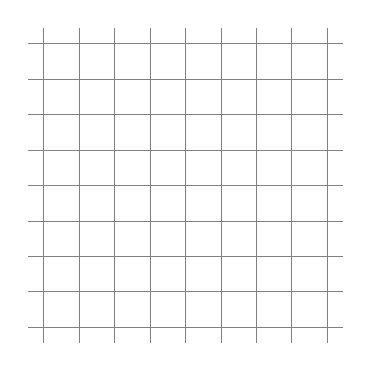
\begin{tikzpicture}
\draw[step=.45cm,gray,very thin] (-2,-2) grid (2,2);
\end{tikzpicture}\end{center}
\begin{center}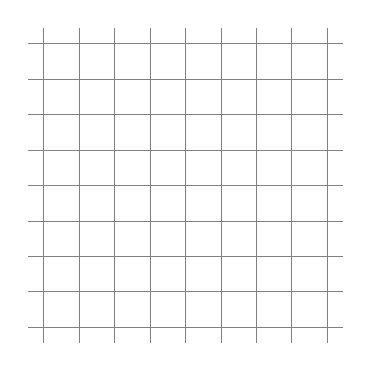
\begin{tikzpicture}
\draw[step=.45cm,gray,very thin] (-2,-2) grid (2,2);
\end{tikzpicture}\end{center}
\begin{center}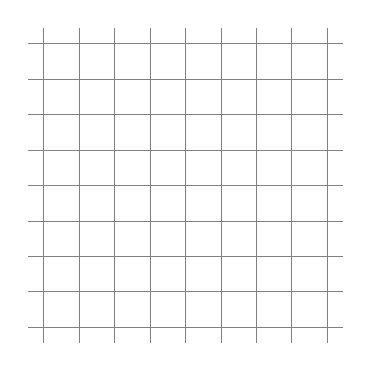
\begin{tikzpicture}
\draw[step=.45cm,gray,very thin] (-2,-2) grid (2,2);
\end{tikzpicture}\end{center}
\end{multicols}




\item Draw the lewis structure of the following compounds and indicate their polarities: \ce{CH4},  \ce{CH2Cl2},  \ce{CHCl3}.
\begin{multicols}{3}
 \begin{center}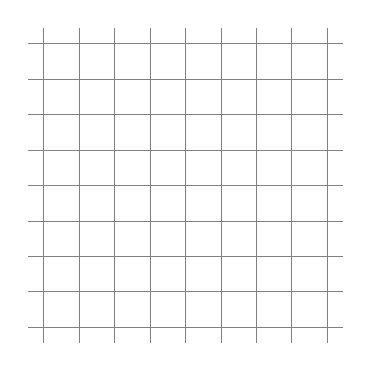
\begin{tikzpicture}
\draw[step=.45cm,gray,very thin] (-2,-2) grid (2,2);
\end{tikzpicture}\end{center}
\begin{center}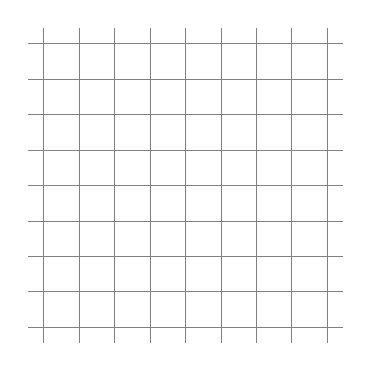
\begin{tikzpicture}
\draw[step=.45cm,gray,very thin] (-2,-2) grid (2,2);
\end{tikzpicture}\end{center}
\begin{center}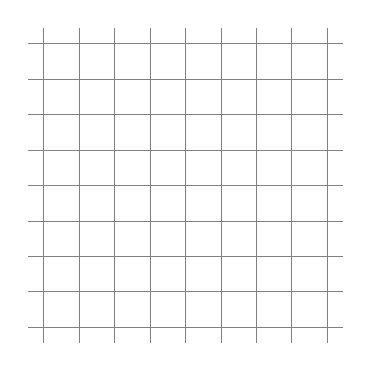
\begin{tikzpicture}
\draw[step=.45cm,gray,very thin] (-2,-2) grid (2,2);
\end{tikzpicture}\end{center}
\end{multicols}



  
\end{enumerate}




\newpage\begin{landscape}
\noindent\begin{center}
\begin{rndtable}{cp{3cm}ccccc}
  \header{Formula} &
  \header{Lewis Structure} &
  \header{\# $e^-$ Regions} &
  \header{Hybridization} &
  \header{Geometry} &
   \header{Angles} &
  \header{Polar?} \\
 \Huge \ce{NH3} \rot{\hspace{1.8cm}} &\Large \begin{centering} \chemfig{\lewis{2:,N}(-[:0]H)(-[:180]H)(-[:270]H)}
\end{centering}
 & \Large 4 & \Large $sp^3$ & \Large Trigonal Pyramidal&\Large$109.5^{\circ}$&\Large Polar\\ [60pt]
\Huge \ce{H2O}\rot{\hspace{1.8cm}} &   &   &   &  & & \\ [60pt]
 \Huge \ce{CH4}\rot{\hspace{1.8cm}}&   &   &   &  & & \\  [60pt]
 \Huge \ce{CH2Cl2}\rot{\hspace{1.8cm}} &   &   &   &  & & \\  [60pt]
\end{rndtable}\end{center}
\end{landscape}


%\newgeometry{right=5cm}
%\thispagestyle{sidebar}
%\sidebar{%
 % \vspace{1em}
 % \vspace{1cm}
 % \vfill
%  \par\vspace*{1em}
%}
%\restoregeometry
\begin{landscape}\begin{center}
\begin{rndtable}{cp{3cm}ccccc}
  \header{Formula} &
  \header{Lewis Structure} &
  \header{\# $e^-$ Regions} &
  \header{Hybridization} &
  \header{Geometry} &
   \header{Angles} &
  \header{Polar?} \\
 \Huge \ce{CO2}\rot{\hspace{1.8cm}}&   &   &   &  & & \\  [60pt]
\Huge \ce{CO3^{2-}}\rot{\hspace{1.8cm}} &   &   &   &  & & \\  [60pt]
 \Huge \ce{CH2O}\rot{\hspace{1.8cm}}&   &   &   &  & & \\  [60pt]
 \Huge \ce{SO2}\rot{\hspace{1.8cm}} &   &   &   &  & & \\  [60pt]
\end{rndtable}\end{center}
\end{landscape}

\begin{landscape}\begin{center}
\begin{rndtable}{cp{3cm}ccccc}
  \header{Formula} &
  \header{Lewis Structure} &
  \header{\# $e^-$ Regions} &
  \header{Hybridization} &
  \header{Geometry} &
   \header{Angles} &
  \header{Polar?} \\
 \Huge \ce{CH3OCH3}\rot{\hspace{1.8cm}} &  \Large \chemfig{C-O-C}    &   &   &  & & \\  [60pt]
\Huge \ce{ICl4^{-}}\small{\hspace{0.05cm}violates octet rule}\rot{\hspace{1.8cm}} &   &   &   &  & & \\  [60pt]
 \Huge \ce{C2H5OH}\rot{\hspace{1.8cm}}& \Large \chemfig{C-C-O}  &   &   &  & & \\  [60pt]
 \Huge \ce{C6H6}\rot{\hspace{1.8cm}} &\Large  \begin{centering} \chemfig{*6(C-C-C-C-C-C-)} \end{centering} &   &   &  & & \\  [60pt]
\end{rndtable}\end{center}
\end{landscape}


\newgeometry{right=5cm}
%\thispagestyle{sidebar}
\sidebar{%
  \vspace{1em}
  \vspace{1cm}
  \vfill
  \par\vspace*{1em}
}
\restoregeometry
\begin{landscape}\begin{center}
\begin{rndtable}{cp{3cm}ccccc}
  \header{Formula} &
  \header{Lewis Structure} &
  \header{\# $e^-$ Regions} &
  \header{Hybridization} &
  \header{Geometry} &
   \header{Angles} &
  \header{Polar?} \\
\Huge \ce{OPCl3\small{\hspace{0.05cm}violates octet rule}}\rot{\hspace{1.8cm}}    &   &   &   &  & & \\  [60pt]
\Huge \ce{PCl5}\small{\hspace{0.05cm}violates octet rule}\rot{\hspace{1.8cm}} &   &   &   &  & & \\  [60pt]
\Huge \ce{AlCl6^{3-}}\small{\hspace{0.05cm}violates octet rule}\rot{\hspace{1.8cm}}     &   &   &   &  & & \\  [60pt]
\Huge \ce{SO4^{2-}}\small{\hspace{0.05cm}violates octet rule}\rot{\hspace{1.8cm}}     & &   &   &  & & \\  [60pt]
\end{rndtable}\end{center}
\end{landscape}

\begin{landscape}\begin{center}
\begin{rndtable}{cp{3cm}ccccc}
  \header{Formula} &
  \header{Lewis Structure} &
  \header{\# $e^-$ Regions} &
  \header{Hybridization} &
  \header{Geometry} &
   \header{Angles} &
  \header{Polar?} \\
\Huge \ce{XeF2}\small{\hspace{0.05cm}violates octet rule}\rot{\hspace{1.8cm}} &   &   &   &  & & \\  [60pt]
\Huge \ce{SF6}\small{\hspace{0.05cm}violates octet rule}\rot{\hspace{1.8cm}} &   &   &   &  & & \\  [60pt]
 \Huge \ce{BrF3}\small{\hspace{0.05cm}violates octet rule}\rot{\hspace{1.8cm}}&   &   &   &  & & \\  [60pt]
 \Huge \ce{SeF4}\small{\hspace{0.05cm}violates octet rule}\rot{\hspace{1.8cm}} &   &   &   &  & & \\ [60pt]
\end{rndtable}\end{center}
\end{landscape}




%%%%%%%%%%%%%HEADING
%\newgeometry{right=5cm}
%\thispagestyle{sidebar}
%\sidebar{%
%  \vspace{1em}
%  \vspace{1cm}
%  \vfill
%  \par\vspace*{1em}
%}
%\restoregeometry
%\clearpage
%\begin{multicols}{2}
%
%\begin{tcolorbox}[enhanced jigsaw,breakable,size=title,
%colback=mybrown!05,colframe=black,fonttitle=\bfseries,
%title=STUDENT INFO,pad at break=1mm, break at=15cm/0pt ]
%\vspace{0.2cm}
%\noindent Name: \rule{5cm}{0.4pt}Date:\rule{1cm}{0.4pt}\\
%Post-lab Done: \tikzcheckmark[scale=2,black]{no mark}\quad
%\end{tcolorbox}
%\end{multicols}
%\hfill
%\vspace{0.2cm}
%\begin{center}
%{\large \bfseries 
%Post-lab Questions 
%\par
%\Huge
%Molecular Geometry
%\\[5pt] \par}
%\vspace{0.2cm}
%\end{center}
%\par
%\noindent
%\uline{  \hfill \normalsize \hfill       }
%
%%%%%%%%%%%%%HEADING
%\begin{enumerate}
%\item Dumas studied mercury with the aim to estimate its molar mass. He found that at 446$^{\circ}$C and 765 torr, 0.812 g of mercury vapor filled a vessel of volume 0.235186 L. From these data, compute the molar mass of mercury.
%\vspace{4cm}
%
%
%\item Calculate the mass of 45.0 L of \ce{NH3} at 27 $^{\circ}$C and 890 mmHg. 
%\vspace{4cm}
%
%
%\item A volume of 30 mL of a gas was collected at a laboratory, in a tube at a temperature
% of 15$^{\circ}$C and 800 mm Hg. The next day at the laboratory was a cooler day.
%The volume of the same gas was 26 mL with the barometer still reading the same pressure. Calculate the laboratory temperature the second day.
%
%\end{enumerate}
%
%
%
%\clearpage\mbox{}\clearpage




 \end{refsection}
\end{document}
